\documentclass[11pt,a4paper]{article}
\usepackage[utf8]{inputenc}
%\usepackage[T1]{fontenc}
\usepackage[czech]{babel}
%\usepackage{amsfonts}
\usepackage{amsthm}
\usepackage{amsmath}
\usepackage{amssymb}
\usepackage[pdftex]{graphicx}
%\usepackage{enumerate}
%\usepackage{stmaryrd}
\usepackage{hyperref}
\usepackage{wasysym}

%\newtheorem{tvrz}{Tvrzení}
%\newtheorem{uloh}{Úloha}
%\newtheorem{lem}[tvrz]{Lemma}

\newcommand{\HRule}{\rule{\linewidth}{0.5mm}}
\newcommand{\cpp}{\textsc{C++}}
\newcommand{\mpp}{\textsc{Matrix++}}
\newcommand{\R}{\mathbb{R}}
\newcommand{\V}{\mathbf{v}}
\newcommand{\x}{\mathbf{x}}

\hyphenation{ma-ti-ce}
%\hyphenation{ša-blo-no-va-nou}
\hyphenation{o-pe-ra-ce}

\renewcommand{\labelitemi}{$\heartsuit$}
\renewcommand{\labelitemii}{$\spadesuit$}
\renewcommand{\labelitemiii}{$\clubsuit$}

\theoremstyle{remark}
\newtheorem{thm}{Theorem}[section]
\newtheorem{note}[thm]{Poznámka}

\begin{document}

\begin{titlepage}
\begin{center}
% Upper part of the page

\includegraphics[viewport=180 50 100 100,scale=0.5]{./logo_mff.jpg}\\[1cm]    

\textsc{\LARGE Matematicko-fyzikální fakulta\\[0.1cm]
Univerzity Karlovy v Praze}\\[1.5cm]

\textsc{\Large Zápočtový program k NPRG041\\ ZS 2012/2013}\\[0.5cm]


% Title
\HRule \\[0.4cm]
{ \huge \bfseries Knihovna \mpp}\\[0.4cm]

\HRule \\[1.5cm]

% Author and supervisor
\begin{minipage}{0.4\textwidth}
\begin{flushleft} \large
\emph{Autor:}\\
Karel~\textsc{Ha}
\end{flushleft}
\end{minipage}
\begin{minipage}{0.4\textwidth}
\begin{flushright} \large
\emph{Cvičící:} \\
RNDr.~F.~\textsc{Zavoral},~Ph. D.
\end{flushright}
\end{minipage}

\vfill
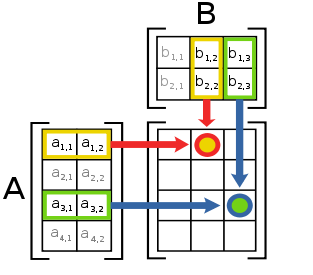
\includegraphics[viewport=140 15 150 65,scale=0.75]{./front.png}\\[1cm]    

% Bottom of the page
{\large \today}

\end{center}

\end{titlepage}

\thispagestyle{empty}

\begin{abstract}
Dokumentace k zápočtovému programu.
Práce je implementací ša\-blo\-no\-va\-né knihovny pro práci s maticemi
representované ve formě kontejnerů jazyka~\cpp.
\end{abstract}

\pagebreak

\thispagestyle{empty}
\tableofcontents

\pagebreak

\setcounter{page}{1}
\pagestyle{headings}

\part{Předmluva}

Text, jenž právě čtete, dokumentuje knihovnu \mpp.
Ta manipuluje s~matematickými maticemi formou kontejnerů programovacího jazyka
C++.
Konkrétně, pro zvolený datový typ a pro zadaný způsob manipulace s prvky
(neboli pro zadané \emph{těleso\/}, nad nímž chceme matici definovat) je skrze
šablony vygenerována jednotlivá třída.

Dále jsou implementovány základní maticové operace: sčítání, odčítání, násobení
skalárem, násobení dvou matic, transposice a další.

Mimojiné je zahrnuta podpora funkcí specifických pro jazyk \cpp: přetí\-že\-ní
operátorů $\ll$ a $\gg$ pro vstupně/výstupní operace; konstruktury a
destruktory kanonické formy; konversní operátory a konstruktory; členské
po\-lož\-ky a~metody splňující normu o~kontejnerech a~iterátorech
\cite{iso-norma}.

Nadto, jakožto praktická aplikace schopností tohoto rozhraní, byl implementován
QR rozklad a~QR algoritmus používáný pro výpočet vlastních čísel.

\pagebreak

\part{Programátorský manuál}
\section{Anotace}
Knihovna pro práci s maticemi.
Nabízí funkce pro běžné maticové operace a rozklady (s možností aplikace např.
QR rozkladu pro hledání vlastních čísel).

\section{Přesné zadání}
Implementace běžných operací s maticemi (sčítání, násobení, inverze,
determinant) použitím efektivních algoritmů. 
Matice bude representována ša\-blo\-no\-va\-nou třídou a bude brát v potaz
zadání jiného tělesa pro prvky.

\section{Struktura Field}

Šablonovaná struktura s~účelem rozhraní pro definici maticového
tělesa.\thinspace%
\footnote{matematické struktury $\mathbb{F} = (0, 1, -, +, \times, ^{-1})$
splňující jisté axiómy (asociativitu, komutativitu, distributivitu a další)}
Hlavička je
\begin{verbatim}
template<typename T> struct Field;
\end{verbatim}

\subsection{Členské atributy}

\begin{itemize}
  \item základní
  \begin{itemize}
    \item \verb=_zero= \ldots neutrální prvek sčítání
    \item \verb=_one= \ldots neutrální prvek násobení
    \item \verb=(*_minus)(const T &)= \ldots inversní prvek vzhledem ke sčítání
    \item \verb=(*_reciprocal)(const T &)= \ldots inversní prvek vzhledem k
      násobení
    \item \verb=(*_plus)(const T &, const T &)= \ldots binární operace sčítání
    \item \verb=(*_times)(const T &, const T &)= \ldots binární operace
      násobení
  \end{itemize}
  \item rozšířené
  \begin{itemize}
    \item \verb=(*_equals)(const T &, const T &)= \ldots rovnost dvou prvků z
      tělesa (např. pro $\mathbb{Z}_p$ se jedná o $a \equiv b \pmod p$)
  \end{itemize}
\end{itemize}

\subsection{Členské metody}

\begin{itemize}
  \item kanonické
  \begin{itemize}
    \item \verb=Field(...)= konstruktor s~parametry $(0, 1, -, ^{-1}, +,
      \times, =)$
  \end{itemize}
  \item pomocné
  \begin{itemize}
    \item \verb=_rec(const T &)= \ldots inversní prvek vzhledem k násobení,
      navíc spustí výjimku \verb=InverseOfNullException= při pokusu o~inversi
      nulového prvku
    \item \verb=subtract(const T &, const T &)= \ldots binární minus jako
      \[
        a - b := a + (-b)
      \]
  \end{itemize}
\end{itemize}

\subsection{Předdefinovaná tělesa}
 
Autor předdefinoval v~souboru \verb=matrix.tpp= následující příklady těles:
\begin{itemize}
  \item \verb=Field<double> fld_reals= \ldots standardní těleso $\R$ definované
    nad~datovým typem \verb=double=
  \item \verb=Field<int> pf= \ldots konečné těleso isomorfní cyklické grupě
    $\mathbb{Z}_p$\thinspace%
    \footnote{z~důvodu efektivity není ovšem kontrolováno, zda-li je $p$
    prvočíslo}
    \begin{itemize}
      \item definované nad~datovým typem \verb=int=
      \item operace jsou prováděny \emph{modulo $p$\/}
      \item invers pro~násobení implementován skrze \emph{Bézoutovy
        koeficienty\/} využitím \emph{Euklidova algoritmu\/}
    \end{itemize}
\end{itemize}

\begin{note}
  Řád konečného tělesa \verb=pf= je nastaven v~souboru~\verb=matrixpp.tpp=
  pomocí proměnné \verb=const int _order_=.
  Těleso je tedy specifikováno \emph{už\/} při překladu.
\end{note}

\section{Třída Matrix}

Nejobecnější kontejner matic - příslušné těleso zadáváno formou jednoho z
atributů.
Hlavička je
\begin{verbatim}
template<typename T=double> class Matrix;
\end{verbatim}
(implicitní \verb=double= jest nastaven pro nejběžnější účely matic nad tělesem
$\R$.)

\subsection{Členské atributy}

\begin{itemize}
  \item soukromé
  \begin{itemize}
    \item \verb=_height= \ldots počet řádků matice
    \item \verb=_width= \ldots počet sloupců matice
    \item \verb=_values= \ldots 1-D pole obsahující samotné prvky matice
  \end{itemize}
  \item veřejné
  \begin{itemize}
    \item \verb=_fld= \ldots ukazatel na maticové těleso
  \end{itemize}
\end{itemize}

\subsection{Členské metody}

\begin{itemize}
  \item veřejné
  \begin{itemize}
    \item \verb=get_height= \ldots vrací počet řádků matice
    \item \verb=get_width= \ldots vrací počet sloupců matice
    \item \verb=at= \ldots vrací hodnotu prvku na zadaných
      indexech\thinspace%
      \footnote{počítáno od $(0,0)$ stejně jako po zbytek textu}
    \item \verb=is_valid= \ldots ověřuje korektnost matice (virtuální funkce:
      vy\-u\-ži\-tel\-né pro potomky třeba při kontrolách rozměrů či
      regularity)
    \item \emph{kanonická část\/} \ldots defaultní konstruktor, operátor
      přiřazení, \uv{copy-constructor}, destruktor
    \item \verb=iterator=, \verb=const_iterator= \ldots iterátory vytvořené
      z~\emph{pointerů\/}
    \item \verb=value_type= \ldots datový typ prvku matice (implicitně:
      \verb=double=)
    \item \verb=reference=, \verb=const_reference= \ldots reference na~prvek
      matice
    \item \verb=difference_type=, \verb=size_type= \ldots paměťová velikost
      prvku matice
    \item \verb=begin=, \verb=cbegin= \ldots prvek levého horního roh matice
    \item \verb=end=, \verb=cend= \ldots konec se nachází
      \emph{za\/}\thinspace%
      \footnote{obdobně jako u všech iterátorů}
      ~prvkem pravého dolního rohu matice
    \item \verb~operator==~, \verb~operator!=~ \ldots porovnání matic: stejné
      rozměry + stejné těleso + prvek po prvku
    \item \verb~swap~ \ldots prohození dvou matic (včetně rozměrů a těles)
    \item \verb~size~, \verb~max_size~ \ldots počet prvků matice (podle
      \verb~_values~)
    \item \verb~empty~ \ldots prázdná matice (\verb=begin= a \verb=end=
      splývají)
    \item \verb~mul_by_scal~ \ldots vynásobení každého prvku matice skalárem
    \item \verb~transpose~ \ldots vrací novou matici jako transposici původní
    \item \verb~subblock~ \ldots vrací souvislou podmatici (při zadání levého
      horního a pravého dolní rohu požadovaného obdélníku)
    \item \verb~column~ \ldots vrací sloupcový vektor matice
    \item \verb~round_to_zeroes~ \ldots vrací matici, v níž jsou prvky blízké
      nule na nulu \uv{za\-o\-krouh\-le\-ny} (pro numerické ustálení
      u~\emph{QR algoritmu\/})
    \item (\verb~LUP~ \ldots \emph{LUP dekomposice\/} stále zbývá
      k~naimplementování)
    \item \verb~QR(SqrMtrx<T> & Q, Matrix & R)~ \ldots vrací \emph{QR
    faktorisaci\/} skrze úpravy referencí na~\verb~Q~ a~\verb~R~.
    \item \verb~operator>>~, \verb~operator<<~ \ldots vstup\thinspace%
      \footnote{zadávají se výška, šířka a samotné prvky matice}
      a výstup z/do~\verb~iostream~ objektu
  \end{itemize}
\end{itemize}

\subsection{Ostatní funkce}

\begin{itemize}
\item Pomocné
  \begin{itemize}
  \item \verb~swap~ \ldots prohození dvou matic (binární zápis namísto
    zápisu unárního)
  \end{itemize}
\item Aritmetické
  \begin{itemize}
  \item \verb~operator+~, \verb~operator-~, \verb~operator*~ \ldots součet,
    rozdíl, součin\thinspace%
    \footnote{metodou dle definice: časová složitost $\mathcal{O}(m \cdot n
    \cdot k)$ pro součin matic o rozměrech $m \times k$ a~$k \times n$.}
    dvou matic
  \end{itemize}
\end{itemize}

\section{Třída Vect}

Veřejný potomek třídy \verb=Matrix=.
Jedná se kontejner sloupcových vektorů, tj.~matic obecně rozměrů $n\times 1$.
Hlavička je
\begin{verbatim}
template<typename T=double> class Vect : public Matrix<T>;
\end{verbatim}

\subsection{Členské atributy}

\begin{itemize}
  \item soukromé
  \begin{itemize}
    \item \verb=_height=, \verb=_width=, \verb=_values= \ldots zděděné po
      třídě~\verb=Matrix=
  \end{itemize}
  \item veřejné
  \begin{itemize}
    \item \verb=_fld= \ldots zděděné po třídě~\verb=Matrix=
  \end{itemize}
\end{itemize}

\subsection{Členské metody}

\begin{itemize}
  \item veřejné
  \begin{itemize}
    \item \verb=begin=, \verb=transpose= \ldots zděděné po třídě~\verb=Matrix=
    \item \verb=is_valid= \ldots kontroluje rozměry (sloupcových vektorů),
      případně spustí výjimku \verb=NotAVectorException=
    \item \emph{kanonická část\/} \ldots defaultní konstruktor, operátor
      přiřazení, \uv{copy-constructor}
    \item \verb=operator Matrix()= \ldots konversní operátor z~\verb=Vect=
      na~\verb=Matrix=
    \item \verb=Vect(const Matrix & m)= \ldots konversní konstruktor
      z~\verb=Matrix= na~\verb=Vect= (s~kontrolou na~rozměry)
    \item \verb=outer_product= \ldots čtvercová matice součinu $\V\V^T$
    \item \verb=inner_product= \ldots matice rozměrů $1\times 1$ součinu
      $\V^T\V$
    \item \verb=norm_squared= \ldots hodnota skalárního součinu
      $\V^T\V$\thinspace%
      \footnote{neboli druhá mocnina $L_2$-normy v~$\R^n$}
    \item \verb=e1_reflection= \ldots reflexe vektoru~$\x$ do~$e_1$, tj.~vektor
      \[
        \begin{bmatrix}
          ||\x|| \\
          0 \\
          \vdots \\
          0
        \end{bmatrix}
      \]
      pro normu $||\cdot||\colon \R^n \to \R$.
      Názorně:

      \begin{center}
      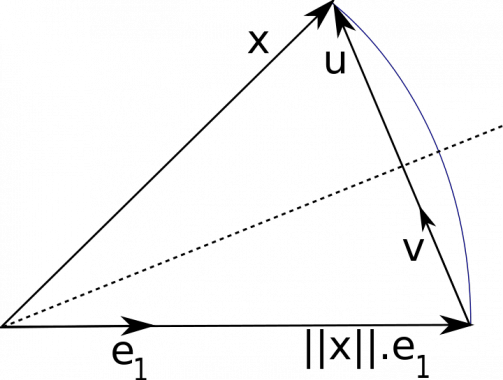
\includegraphics[width=0.4\textwidth]{./householder_reflection.png}
      \end{center}

      (Implementováno pro šablonu se~specializovaným typem \verb=double=.)
    \item \verb=Householder= \ldots matice \emph{Householderovy reflexe\/}
      \[
        \mathbf{H}(\V) = \mathbf{I}_n - \frac{2}{\V^T\V}\V\V^T
      \]
    \item \verb=Householder_canon= \ldots matice zobrazující $\V$ do vektoru
      z~metody \verb=e1_reflection=\thinspace%
      \footnote{konkrétně $||\V||\cdot \mathbf{e}_1$}
      \[
        \mathbf{H} :=
        \begin{cases}
          \mathbf{I}_n &\mbox{iff } \V = ||\V||\cdot \mathbf{e}_1 \\
          \mathbf{H}(\V - ||\V||\cdot \mathbf{e}_1) & \mbox{jinak}
        \end{cases}
      \]
  \end{itemize}
\end{itemize}

\section{Třída SqrMtrx}

Veřejný potomek třídy \verb=Matrix=.
Jedná se kontejner čtvercových matic, tj.~matic obecně rozměrů $n\times n$.
Hlavička je
\begin{verbatim}
template<typename T=double> class SqrMtrx : public Matrix<T>;
\end{verbatim}

\subsection{Členské atributy}

\begin{itemize}
  \item soukromé
  \begin{itemize}
    \item \verb=_height=, \verb=_width=, \verb=_values= \ldots zděděné po
      třídě~\verb=Matrix=
  \end{itemize}
  \item veřejné
  \begin{itemize}
    \item \verb=_fld= \ldots zděděné po třídě~\verb=Matrix=
  \end{itemize}
\end{itemize}

\subsection{Členské metody}

\begin{itemize}
  \item veřejné
  \begin{itemize}
    \item \verb=begin=, \verb=transpose= \ldots zděděné po třídě~\verb=Matrix=
    \item \verb=is_valid= \ldots kontroluje rozměry (čtvercových matic),
      případně spustí výjimku \verb=NotASqrMtrxException=
    \item \emph{kanonická část\/} \ldots defaultní konstruktor, operátor
      přiřazení, \uv{copy-constructor}
    \item \verb=operator Matrix()= \ldots konversní operátor ze~\verb=SqrMtrx=
      na~\verb=Matrix=
    \item \verb=SqrMtrx(const Matrix & m)= \ldots konversní konstruktor
      z~\verb=Matrix= na~\verb=SqrMtrx= (s~kontrolou na~rozměry)
    \item \verb=QR_algorithm= \ldots spuštění \emph{QR metody\/} \cite{qr-meth}
      na~aktuální objekt matice čtvercových rozměrů při~zadaném počtu iterací
  \end{itemize}
\end{itemize}

\section{Výjimky}

Knihovna využívá vlastní hierarchii výjimek.

Seznam použitých výjimek:

\begin{itemize}
  \item veřejní potomci třídy \verb=exception=
  \begin{itemize}
    \item \verb=InverseOfNullException= \ldots při inversi nulového prvku
    \item \verb=MismatchedDimException= \ldots při chybě v~rozměrech matice
    \item \verb=MismatchedFieldException= \ldots při neshodujících se
      rozhraních pro tělesa
    \item \verb=OutOfRangeException= \ldots při indexech mimo rozměry matice
  \end{itemize}
  \item veřejní potomci třídy \verb=MismatchedDimException=
  \begin{itemize}
    \item \verb=NotAVectorException= \ldots při rozměrech různých $n \times 1$
    \item \verb=NotASqrMtrxException= \ldots při rozměrech různých $n \times n$
  \end{itemize}
\end{itemize}

\pagebreak

\part{Uživatelský manuál}
Pro účely názorné ukázky knihovny \mpp byly sepsány testovací programy pro
demonstraci jednotlivých funkcionalit.
Tyto se nacházejí v~souborech tvaru \verb=[jmeno].cpp= a s~pomocí přiloženého
\verb=Makefile= je lze přeložit příkazy tvaru
\begin{verbatim}
$ make [jmeno].exe
\end{verbatim}

\section{Program io.exe} \label{io.exe}

Tato část testuje vstupně/výstupní operace.
Na standardním vstupu (pomocí objektu \verb=cin=) přijme následující údaje o
matici:
\begin{itemize}
\item počet řádků $m$
\item počet sloupců $n$
\item hodnoty jednotlivých položek $a_{i,j}$ (po řádcích, zleva doprava)
\end{itemize}
Na standardní výstup (pomocí objektu \verb=cout=) vypíše hodnoty matice
ve~tvaru:
\[
  \begin{bmatrix}
    a_{1,1} & a_{1,2} & \cdots & a_{1,n} \\
    a_{2,1} & a_{2,2} & \cdots & a_{2,n} \\
    \vdots  & \vdots  & \ddots & \vdots  \\
    a_{m,1} & a_{m,2} & \cdots & a_{m,n}
  \end{bmatrix}
\]

\section{Program arithmetics.exe}

Program demonstruje elementární a~některé pomocné operace nad~maticemi:
Nejprve jsou zadány vstupní matice (formát viz Sekce~\ref{io.exe}\thinspace):
\begin{enumerate}
\item celočíselná matice $A$ (nad tělesem $\mathbb{Z}_5$ při hodnotě proměnné
  \verb~_order_ = 5~)
\item reálná matice $B$ (nad tělesem $\mathbb{R}$)
\item celočíselná matice $C$ (nad tělesem $\mathbb{Z}_5$ při hodnotě proměnné
  \verb~_order_ = 5~)
\item reálná matice $D$ (nad tělesem $\mathbb{R}$)
\item celočíselná matice $E$ (nad tělesem $\mathbb{Z}_5$ při hodnotě proměnné
  \verb~_order_ = 5~)
\end{enumerate}
Dále jsou předvedeny následující funkce:
\begin{enumerate}
\item \verb~empty()~ \ldots ověří (ne)prázdnost matice $B$
\item \verb~mul_by_scal(-1)~ \ldots matice $A$ s~opačnými znaménky
\item \verb~swap()~ \ldots výměna obsahu matic $A$ a~$C$
\item \verb~operator+~ \ldots $A+C$, $B+D$
\item \verb~operator-~ \ldots $A-C$, $B-D$
\item \verb~subblock(1, 1, 2, 3)~ \ldots podmatice matice $B$:
\[
  \begin{bmatrix}
    b_{1,1} & b_{1,2} & b_{1,3} \\
    b_{2,1} & b_{2,2} & b_{2,3}
  \end{bmatrix}
\]
\item \verb~subblock(2, 1, 4, 4)~ \ldots podmatice matice $B$:
\[
  \begin{bmatrix}
    b_{2,1} & b_{2,2} & b_{2,3} & b_{2,4} \\
    b_{3,1} & b_{3,2} & b_{3,3} & b_{3,4} \\
    b_{4,1} & b_{4,2} & b_{4,3} & b_{4,4}
  \end{bmatrix}
\]
\item \verb~column(i)~ \ldots všechny sloupce matice $B$
\item \verb~operator!=, operator==~ \ldots $B \ne D$, $A = E$
\item \verb~size(), max_size()~ \ldots počet prvků $A, B$
\item \verb~const_iterator~ \ldots ukázka manipulace s~iterátory
\item \verb~transpose()~ \ldots transposice matice $E$
\end{enumerate}

\clearpage

\begin{verbatim}
---------------------------------------------------------------
Choose option (enter the part in brackets)
(S)ym            - symmetrization
(D)ijkstra       - shortest path between node & other nodes
(F)loyd-Warshall - shortest path between every 2 nodes
tar(J)an         - strongly connected components
(T)sort          - topological ordering
(C)losure        - transitive closure
(R)eduction      - transitive reduction
l(I)st-convert   - from adjacency matrix to list of successors
(M)atrix-convert - from list of successors to adjacency matrix
c(L)ear          - clear screen (only for in *nix like OS) 
Displa(Y)        - display the graph 
(H)elp           - display this menu:) 
(Q)uit           - quit the program 
---------------------------------------------------------------
>>
\end{verbatim}

Jak vidno, tuto nabídku lze kdykolit znova vyvolat pomocí
příkazu {\tt h}:%
\footnote{Příkazy lze zadávat velkými i malými písmeny abecedy.
Dokonce ani nevadí, když jsou za prvním písmenem další znaky, ty se až do konce
  řádku ignorují.}

\begin{verbatim}
>> h 
\end{verbatim}

\section{Vstup a příkazy programu}
\subsection{Sym}
Příkaz, jenž \uv{zorientuje každou hranu na obě strany}, dokáže i zajistit
převod orientovaného grafu na neorientovaný.

\begin{verbatim}
>> s
List of successor representation:
1. node -> 3(3.140000)
3. node -> 1(3.140000)
Matrix representation:
----    ----    3.14
----    ----    ----
3.14    ----    ----
\end{verbatim}

{\noindent \sl Pozn.~Vstup z \tt testing/sym2.in}

\subsection{Dijkstra}
Příkaz spuštění {\sl Dijkstrova algoritmu\/} ze zadaného vrcholu.

\begin{verbatim}
>> d
Enter starting node of graph: 1
From 1.node to all nodes respectively:
0.000000 7.000000 9.000000 20.000000 20.000000 11.000000 
\end{verbatim}

{\noindent \sl Pozn.~Vstup z \tt testing/dijkstra2.in}

\subsection{Floyd-Warshall}
Příkaz spuštění {\sl Floyd-Warshallova algoritmu\/}.%
\footnote{Mimochodem tento algoritmus je použit pro vytvoření grafu
transitivního uzávěru v representaci se seznamem následovníků.
Autor tak učinil z dvou prostých důvodů: zaprvé Floyd-Warshall podává lepší
informaci o vahách mezi vrcholy jakožto jejich vzdálenosti; zadruhé algoritmus
transitivního uzávěru je jen upravená verse Floyd-Warshallova algoritmu \sl :-)}


\begin{verbatim}
>> f
List of successor representation (i.e., transitive closure):
1. node -> 4(3.600000) 2(1.200000) 1(1.100000)
2. node -> 4(2.400000)
3. node -> 4(6.700000) 2(4.300000) 1(3.100000)
Matrix representation:
1.10    1.20    ----    3.60
----    0.00    ----    2.40
3.10    4.30    0.00    6.70
----    ----    ----    0.00
\end{verbatim}

{\noindent \sl Pozn.~Vstup z \tt testing/floyd\_warshall.in}

\subsection{Tarjan}
Příkaz spuštění {\sl Tarjanova algoritmu\/}.%
\footnote{Počínaje od vrcholu s indexem 1, neb hlavní procedura zkoumá
  nezpracované vrcholy v rostoucím pořadí indexů.}%
\footnote{Tarjanův algoritmus zároveň určuje reversní topologické uspořádání
  grafu komponent zadaného grafu.}

\begin{verbatim}
>> j
( 7 6 )
( 8 4 3 )
( 5 2 1 )
\end{verbatim}

{\noindent \sl Pozn.~Vstup z \tt testing/scc2.in}

\subsection{TSort}
Příkaz spuštění algoritmu pro nalezení {\sl topologického uspořádání\/}.%
\footnote{V případě neexistence takového uspořádání (nastane právě v grafech s
  cykly) se vypíše \tt NOT AN ACYCLIC GRAPH!}

\begin{verbatim}
>> t
Topological ordering: 1 4 2 3 5
\end{verbatim}

{\noindent \sl Pozn.~Vstup z \tt testing/tsort.in}

\subsection{Closure}
Příkaz spuštění algoritmu pro vytvoření {\sl transitivního uzávěru\/}.%
\footnote{Zde použitá implementace funkce vrací matici sousednosti nalezeného
  uzávěru.
Ovšem knihovna poskytuje funkci {\tt listConvertBit}, jež matici dokáže převést
  na representaci se seznamem následovníků.
To je náležitě využito v {\tt main.c} pro zobrazení obou možných representací,
  jak si lze prohlédnout v přiloženém výstupu.}

\begin{verbatim}
>> c
List of successor representation:
1. node -> 5(1.000000) 4(1.000000) 3(1.000000) 2(1.000000) 1(1.000000)
2. node -> 5(1.000000) 3(1.000000) 2(1.000000)
3. node -> 5(1.000000) 3(1.000000)
4. node -> 5(1.000000) 4(1.000000) 3(1.000000)
5. node -> 5(1.000000)
Matrix representation:
1 1 1 1 1 
0 1 1 0 1 
0 0 1 0 1 
0 0 1 1 1 
0 0 0 0 1 
\end{verbatim}

{\noindent \sl Pozn.~Vstup z \tt testing/closure.in}

\subsection{Reduction}
Příkaz spuštění algoritmu pro vytvoření {\sl transitivního redukce.
\vskip .45cm
Pozn.~Tato implementace zvládá nalézt redukci {\bf pouze} v acyklických grafech.
Autor z důvodů časové tísně a značné vyspělosti obecného algoritmu nebyl
schopen vyřešit případ pro grafy s cykly a slibuje, že se do přístě napraví
\sl :-)}
\vskip .45cm

Výstup toho příkazu je k nalezení na další stránce $\dots$

\vfil\eject

\begin{verbatim}
>> r
List of successor representation:
1. node -> 4(1.000000) 2(1.000000)
2. node -> 3(1.000000)
3. node -> 5(1.000000)
4. node -> 3(1.000000)
Matrix representation:
0 1 0 1 0 
0 0 1 0 0 
0 0 0 0 1 
0 0 1 0 0 
0 0 0 0 0 
\end{verbatim}

{\noindent \sl Pozn.~Vstup z \tt testing/reduction2.in}

\begin{verbatim}
>> r
Warning! Given graph is NOT acyclic.
The result of transitive reduction is ungranted!
List of successor representation:
1. node -> 2(1.000000)
2. node -> 3(1.000000)
3. node -> 1(1.000000)
4. node -> 5(1.000000)
5. node -> 6(1.000000)
6. node -> 4(1.000000)
Matrix representation:
0 1 0 0 0 0 
0 0 1 0 0 0 
1 0 0 0 0 0 
0 0 0 0 1 0 
0 0 0 0 0 1 
0 0 0 1 0 0 
\end{verbatim}

{\noindent \sl Pozn.~Vstup z \tt testing/reduction\_cyclic.in}

\subsection{List-convert}
Příkaz spuštění pro převod {\sl maticové \rm representace na representaci se
  \sl seznamem následovníků\/}.%
\footnote{Příkaz dokáže fungovat obecně.
Pro účely jednoduchosti však {\sl main.c} využívá funkci tak, že seznam
  následovníků nejprve převede na matici a ta se pomocí {\sl list-convert}
  převede zpět.
Samozřejmě je list-convert využit ještě u funkcí vracející maticové
  representací jakými jsou například {\tt closure\/ {\rm či} reduction\/}.
}
\vfil\eject
\begin{verbatim}
>> i
Converting the already matrix-converted graph
  to list-of-sucessors representation...
1. node -> 4(0.200000) 3(0.600000) 2(0.200000)
2. node -> 3(0.300000)
3. node -> 5(0.500000)
4. node -> 5(0.800000) 3(0.200000)
\end{verbatim}

{\noindent \sl Pozn.~Vstup z \tt testing/list\_convert.in}

\subsection{Matrix-convert}
Příkaz spuštění pro převod se {\sl seznamem následovníků \rm representace na
  representaci \sl maticovou\/}.%
\footnote{Příkaz dokáže fungovat obecně.
Pro účely jednoduchosti však {\tt main.c} využívá funkci tak, že seznam
  následovníků nejprve převede na matici a ta se pomocí {\tt list-convert}
  převede zpět.
Samozřejmě je list-convert využit ještě u funkcí vracející maticové
  representací jakými jsou například {\tt closure či \tt reduction\/}.
}

\begin{verbatim}
>> m

----    0.20    0.60    0.20    ----
----    ----    0.30    ----    ----
----    ----    ----    ----    0.50
----    ----    0.20    ----    0.80
----    ----    ----    ----    ----
\end{verbatim}

{\noindent \sl Pozn.~Vstup z \tt testing/matrix\_convert.in}

\subsection{Display}
Příkaz pro zobrazení grafu v representaci se seznamem následovníků.

\noindent {\bf Formát:}

\noindent {\sl $<$index výchozího uzlu$>$\tt.node -> \sl $<$index příchozího
  uzlu$>$\tt (\sl$<$váha$>$\tt)}

\begin{verbatim}
>> y
1. node -> 4(0.200000) 3(0.600000) 2(0.200000)
2. node -> 3(0.300000)
3. node -> 5(0.500000)
4. node -> 5(0.800000) 3(0.200000)
\end{verbatim}

\subsection{Clear}
Příkaz na vyčištění obrazovky (v abstraktním slova smyslu, samozřejmě, jinak
použijte suchý hadřík či látku {\tt :-)}
Funguje převážně na systémech *nixového typu, páč využívá systémové procedury
\verb=clear=.

\begin{verbatim}
>> l
\end{verbatim}

\subsection{Quit}
A tady končí naše cesta...

\begin{verbatim}
>> q
Bye bye...
\end{verbatim}

\pagebreak

\part{Závěr}

Nabízí se nemalé množství prostoru pro vylepšení:
\begin{enumerate}
  \item {\bf Násobení matic\/} přímo podle definice není nejefektivnější.
    Lze vylepšit přepsáním funkce
\begin{verbatim}template<typename T>
Matrix<T> operator*(const Matrix<T> &, const Matrix<T> &);\end{verbatim}
    např. pomocí \emph{Strassenova algoritmu\/}.
  \item {\bf LUP rozklad\/} byl vynechán, neboť jeho využitelnost je možno
    do\-sta\-teč\-ně uspokojivě nahradit \emph{QR rozkladem\/}.
    Přesto však autor vřele uvítá jakékoli snahy o~toto rozšíření.
\end{enumerate}

\pagebreak

\begin{thebibliography}{9}

\bibitem{iso-norma}
Norma \textsc{ISO/IEC N3290} programovacího jazyka \cpp.

\bibitem{qr-meth}
  {\sc Kublanovskaya}, Vera N.
  On some algorithms for the solution of the complete eigenvalue problem.
  In: \emph{USSR Computational Mathematics and Mathematical Physics\/}.
  1963,
  no.~3,
  vol.~8,
  pp.~637-657.

\end{thebibliography}

\end{document}
